\chapter{Materials \& Methods}

%\textbf{This section should include a recipe of what you did (explain what you have done so if someone wants to reproduce the experiment, they can).  A flow chart is typically helpful.  Also, make sure to define all software that you used including version numbers and OS.  Should also include a description of statistical methods used (if any).\footnote{For more information see: \url{http://rc.rcjournal.com/content/49/10/1229.short}}}

For this \ac{IAPT} a multi-stage approach was used for data collection, analyses and evaluation.
This approach is described in figure~\ref{fig:flowchart} as a flowchart.

\begin{figure}[h!]
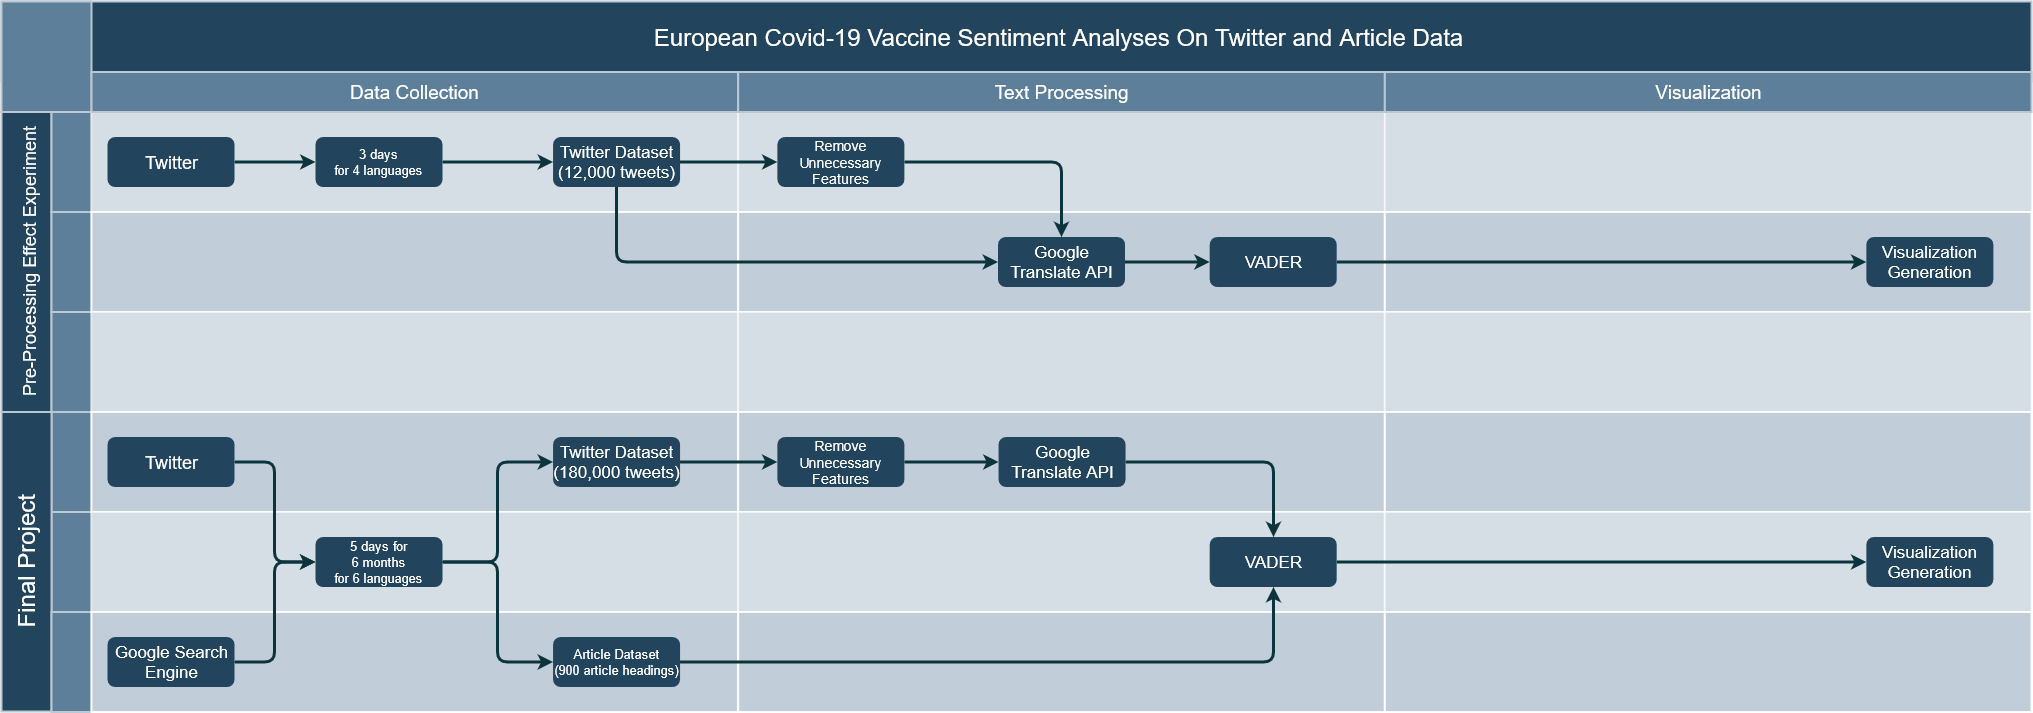
\includegraphics[scale=0.2]{IAPT Flowchart}
\caption[Method Flowchart]{Flowchart of the Method of Experiment\index{Method Flowchart}}
\label{fig:flowchart}
\end{figure}


% Maybe not for motivation
%To focus the analyses on European countries and citizens tweets where collected in 6 languages: English, Spanish, French, German, Italian and Dutch.
%The data was collected over a range of 30 dates spanning 6 months from December 2020 till May 2021.
%To diversify the data collected from Twitter 900 articles where also collected that where written about the Covid-19 pandemic.
%Articles where collected for 6 countries: United Kingdom, Spain, France, Germany, Italy, Netherlands, and over the same date range as the Twitter dataset.

\section{Data Collection}

\subsection{Twitter Dataset}

The large scale dataset of tweets maintained by \citet{banda2020largescale} is very large and analysing it in its entirety would be expensive, lengthy and out of scope for this \ac{IAPT}, since the majority of the data present is generated outside of the \ac{EU} borders.
The dataset contains daily folders representing each each day from the 22nd of March 2020, which contain two files, one of all tweets and retweets on the day, and the other a cleaned version with no retweets.
Instead all of this available data for every month from December 2020 till May 2021, 5 dates, the 1st, 7th, 14th, 21st, 28th where chosen and the clean dataset file was used.
It was decided that 1000 tweets from 6 languages would suffice to form the Twitter dataset.
The 6 languages, English, Spanish, French, German, Italian and Dutch are the European languages with the most presence in the Panacea Lab dataset.
An important point to consider when using the Panacea Lab dataset is that only the Tweet ID is available.
However this ID can be easily used to download and collect the Tweet text and other Tweet features.
For this \ac{IAPT} the Python library, Tweepy a Python wrapper for the Twitter \ac{API} was used ~\citep{roesslein2020tweepy}.
The use of the Twitter \ac{API} requires the signing-up to the service with Twitter, where after approval \ac{API} are shared.
The free version comes with limitations such as a limit of 300 lookups/ 15 minutes, however a limit on status retrieval through the ID does not exist.
Hence for this part of the data collection no limitations were imposed by the Twitter \ac{API}.
In total 180,000 tweets where collected.

A smaller dataset was also collected following the same method as described above.
This smaller dataset features a 1000 Tweets from 3 dates, the 1st of January, February and March and 4 languages, English, Spanish, French, German.
This dataset was used to test the effect of pre-processing the tweets before passing them to a \ac{VADER} model.
In total 12,000 tweets where collected.

\subsection{Article Dataset}

As the focus of this \ac{API} was explained to be more directed towards using social media data, it was decided that the article dataset would be much smaller in scale.
Using the Google search engine a query was done for every day a file was taken from the Panacea Lab dataset.
The query was of the format: \textquote{{Country} Covid* before:{Date in YYYY-MM-DD Format} After:{Day before Date in YYYY-MM-DD Format}}
5 relevant articles where collected for each day and stored in a number of csv files.
In total 900 articles where collected.

\section{Data Processing}
asd

\section{Sentiment Analyses}
asd

\section{Visualization}
asd